\def\paperversiondraft{draft}
\def\paperversionnormal{normal}

% If the paper version is set to 'normal' mode keep it,
% otherwise set it to 'draft' mode.
\ifx\paperversion\paperversionnormal
\else
  \def\paperversion{draft}
\fi

\documentclass[a4paper]{scrartcl}

\usepackage{colortbl}

% 'draftonly' environment
\usepackage{environ}
\ifx\paperversion\paperversiondraft
\newenvironment{draftonly}{}{}
\else
\NewEnviron{draftonly}{}
\fi

% Most PL conferences are edited by conference-publishing.com. Follow their
% advice to add the following packages.
%
% The first enables the use of UTF-8 as character encoding, which is the
% standard nowadays. The second ensures the use of font encodings that support
% accented characters etc. (Why should I use this?). The mictotype package
% enables certain features 'to­wards ty­po­graph­i­cal per­fec­tion
\usepackage[utf8]{inputenc}
\usepackage[T1]{fontenc}
\usepackage{microtype}

\usepackage{xargs}
\usepackage{lipsum}
\usepackage{xparse}
\usepackage{xifthen, xstring}
\usepackage{xspace}
\usepackage{marginnote}
\usepackage{etoolbox}
\usepackage[acronym,shortcuts]{glossaries}
\usepackage{hyperref}

% \usepackage[numbers]{natbib} % for \citeauthor

%%%%%%%%%%%%%%%%%%%%%%%%%%%%%%%%%%%%%%%%%%%%%%%%%%%%%%%%%%%%%%%%%%%%%%%%%%%%%%%
% Broaden margins to make room for todo notes
%%%%%%%%%%%%%%%%%%%%%%%%%%%%%%%%%%%%%%%%%%%%%%%%%%%%%%%%%%%%%%%%%%%%%%%%%%%%%%%

\makeatletter
\patchcmd{\@addmarginpar}{\ifodd\c@page}{\ifodd\c@page\@tempcnta\m@ne}{}{}
\makeatother
\ifx\paperversion\paperversiondraft
  \makeatletter
  \if@ACM@journal
    \geometry{asymmetric}
    \paperwidth=\dimexpr \paperwidth + 3.5cm\relax
    \oddsidemargin=\dimexpr\oddsidemargin + 0cm\relax
    \evensidemargin=\dimexpr\evensidemargin + 0cm\relax
    \marginparwidth=\dimexpr \marginparwidth + 3cm\relax
    \setlength{\marginparwidth}{4.6cm}
    % This makeatletter box helps to move notes to the right
    \makeatletter
    \long\def\@mn@@@marginnote[#1]#2[#3]{%
      \begingroup
        \ifmmode\mn@strut\let\@tempa\mn@vadjust\else
          \if@inlabel\leavevmode\fi
          \ifhmode\mn@strut\let\@tempa\mn@vadjust\else\let\@tempa\mn@vlap\fi
        \fi
        \@tempa{%
          \vbox to\z@{%
            \vss
            \@mn@margintest
            \if@reversemargin\if@tempswa
                \@tempswafalse
              \else
                \@tempswatrue
            \fi\fi
            %\if@tempswa
              \rlap{%
                \if@mn@verbose
                  \PackageInfo{marginnote}{xpos seems to be \@mn@currxpos}%
                \fi
                \begingroup
                  \ifx\@mn@currxpos\relax\else\ifx\@mn@currxpos\@empty\else
                      \kern-\dimexpr\@mn@currxpos\relax
                  \fi\fi
                  \ifx\@mn@currpage\relax
                    \let\@mn@currpage\@ne
                  \fi
                  \if@twoside\ifodd\@mn@currpage\relax
                      \kern\oddsidemargin
                    \else
                      \kern\evensidemargin
                    \fi
                  \else
                    \kern\oddsidemargin
                  \fi
                  \kern 1in
                \endgroup
                \kern\marginnotetextwidth\kern\marginparsep
                \vbox to\z@{\kern\marginnotevadjust\kern #3
                  \vbox to\z@{%
                    \hsize\marginparwidth
                    \linewidth\hsize
                    \kern-\parskip
                    \marginfont\raggedrightmarginnote\strut\hspace{\z@}%
                    \ignorespaces#2\endgraf
                    \vss}%
                  \vss}%
              }%
          }%
        }%
      \endgroup
    }
    \makeatother
  \else
    \paperwidth=\dimexpr \paperwidth + 6cm\relax
    \oddsidemargin=\dimexpr\oddsidemargin + 3cm\relax
    \evensidemargin=\dimexpr\evensidemargin + 3cm\relax
    \marginparwidth=\dimexpr \marginparwidth + 3cm\relax
    \setlength{\marginparwidth}{4.6cm}
  \fi
  \makeatother
\fi

%%%%%%%%%%%%%%%%%%%%%%%%%%%%%%%%%%%%%%%%%%%%%%%%%%%%%%%%%%%%%%%%%%%%%%%%%%%%%%%
% Add \createtodoauthor command
%%%%%%%%%%%%%%%%%%%%%%%%%%%%%%%%%%%%%%%%%%%%%%%%%%%%%%%%%%%%%%%%%%%%%%%%%%%%%%%

\usepackage[textsize=tiny]{todonotes}
\usepackage[normalem]{ulem}

\makeatletter
\font\uwavefont=lasyb10 scaled 652
\newcommand\colorwave[1][blue]{\bgroup\markoverwith{\lower3\p@\hbox{\uwavefont\textcolor{#1}{\char58}}}\ULon}

\newcommand\highlight[2]{{\color{#1}{\colorwave[#1]{#2}}}}
\makeatother

\makeatletter
\newcommand\InFloat[2]{\ifnum\@floatpenalty<0\relax#1\else#2\fi}
\makeatother

\ifx\paperversion\paperversiondraft
\newcommand\createtodoauthor[2]{
  \def\tmpdefault{emptystring}
  \expandafter\newcommand\csname #1\endcsname[2][\tmpdefault]{% comment to avoid spurious whitespace
    \def\tmp{##1}% comment to avoid spurious whitespace
    \InFloat{
        \smash{
	  \marginnote{
	    \todo[inline,linecolor=#2,backgroundcolor=#2,bordercolor=#2]
	      {\textbf{#1 (Figure):} ##2}
          }
        }
    }{\ifthenelse{\equal{\tmp}{\tmpdefault}} % Is there text to highlight?
      {\todo[linecolor=#2,backgroundcolor=#2,bordercolor=#2]{\textbf{#1:} ##2}\ignorespaces}
      {\ifthenelse{\equal{##2}{}} % Is there a note?
        {\highlight{#2}{##1}}
        {\highlight{#2}{##1}\todo[linecolor=#2,backgroundcolor=#2,bordercolor=#2]
	  {\textbf{#1:} ##2}% comment to avoid spurious whitespace
	}% comment to avoid spurious whitespace
      }% comment to avoid spurious whitespace
    }% comment to avoid spurious whitespace
  }
}
\else
\newcommand\createtodoauthor[2]{%
\expandafter\newcommand\csname #1\endcsname[2][]{##1}%
}%
\fi

%%%%%%%%%%%%%%%%%%%%%%%%%%%%%%%%%%%%%%%%%%%%%%%%%%%%%%%%%%%%%%%%%%%%%%%%%%%%%%%
% Add minted and support custom lexers
%%%%%%%%%%%%%%%%%%%%%%%%%%%%%%%%%%%%%%%%%%%%%%%%%%%%%%%%%%%%%%%%%%%%%%%%%%%%%%%
\usepackage{minted}
\usepackage{etoolbox}

\makeatletter
\ifcsdef{minted@optlistcl@quote}
{
\ifwindows
  \renewcommand{\minted@optlistcl@quote}[2]{%
    \ifstrempty{#2}{\detokenize{#1}}{\detokenize{#1="#2"}}}
\else
  \renewcommand{\minted@optlistcl@quote}[2]{%
    \ifstrempty{#2}{\detokenize{#1}}{\detokenize{#1='#2'}}}
\fi

% similar to \minted@def@optcl@switch
\newcommand{\minted@def@optcl@novalue}[2]{%
  \define@booleankey{minted@opt@g}{#1}%
    {\minted@addto@optlistcl{\minted@optlistcl@g}{#2}{}%
     \@namedef{minted@opt@g:#1}{true}}
    {\@namedef{minted@opt@g:#1}{false}}
  \define@booleankey{minted@opt@g@i}{#1}%
    {\minted@addto@optlistcl{\minted@optlistcl@g@i}{#2}{}%
     \@namedef{minted@opt@g@i:#1}{true}}
    {\@namedef{minted@opt@g@i:#1}{false}}
  \define@booleankey{minted@opt@lang}{#1}%
    {\minted@addto@optlistcl@lang{minted@optlistcl@lang\minted@lang}{#2}{}%
     \@namedef{minted@opt@lang\minted@lang:#1}{true}}
    {\@namedef{minted@opt@lang\minted@lang:#1}{false}}
  \define@booleankey{minted@opt@lang@i}{#1}%
    {\minted@addto@optlistcl@lang{minted@optlistcl@lang\minted@lang @i}{#2}{}%
     \@namedef{minted@opt@lang\minted@lang @i:#1}{true}}
    {\@namedef{minted@opt@lang\minted@lang @i:#1}{false}}
  \define@booleankey{minted@opt@cmd}{#1}%
      {\minted@addto@optlistcl{\minted@optlistcl@cmd}{#2}{}%
        \@namedef{minted@opt@cmd:#1}{true}}
      {\@namedef{minted@opt@cmd:#1}{false}}
}
\minted@def@optcl@novalue{customlexer}{-x}
}
{
}
\makeatother

\usepackage{tikz}
\usetikzlibrary{arrows}
\usetikzlibrary{shapes}

%%%%%%%%%%%%%%%%%%%%%%%%%%%%%%%%%%%%%%%%%%%%%%%%%%%%%%%%%%%%%%%%%%%%%%%%%%%%%%%
% Base style and command for \circled to print a colored circle
%%%%%%%%%%%%%%%%%%%%%%%%%%%%%%%%%%%%%%%%%%%%%%%%%%%%%%%%%%%%%%%%%%%%%%%%%%%%%%%
% Width is assured to be the same across all characters using the typewriter font which is monospaced
% Zeroing out the inner separator removes padding between content and node (inner sep).
% Zeroing out the outer separator removes space between the node border and its anchors (e.g., east).
% Minimum size was derived on experimentation and it may need adjustment when changing font style/size.
%
% There is no guarantee for the letter ascenders/descenders to baseline when set to char.base, hence adding \strut.
% which is an invisible vertical rule with the height and depth of the parentheses ( and ).
% It ensures that the line height in a line of text is at least as large as if it contained parentheses. 
\tikzset{
  circledstyle/.style={
    shape=circle,
    #1,
    font=\tt\small,
    inner sep=0pt,
    outer sep=0pt,
    minimum size=1.2em,
    text=black
  }
}

% define a base tikz node for circled commands accepting a fill colour and the node text as arguments
\DeclareRobustCommand{\circledbase}[3][]{%
    \tikz[baseline=(char.base)]{\node[circledstyle, fill=#2] (char) {#3\strut};}%
}


% \ifx\acmversion\acmversionjournal
  %% Journal information (used by PACMPL format)
  %% Supplied to authors by publisher for camera-ready submission
  \acmJournal{PACMPL}
  \acmVolume{1}
  \acmNumber{1}
  \acmArticle{1}
  \acmYear{2017}
  \acmMonth{1}
  \acmDOI{10.1145/nnnnnnn.nnnnnnn}
  \startPage{1}
\else
  %% Conference information (used by SIGPLAN proceedings format)
  %% Supplied to authors by publisher for camera-ready submission
  \acmConference[PL'17]{ACM SIGPLAN Conference on Programming Languages}{January 01--03, 2017}{New York, NY, USA}
  \acmYear{2017}
  \acmISBN{978-x-xxxx-xxxx-x/YY/MM}
  \acmDOI{10.1145/nnnnnnn.nnnnnnn}
  \startPage{1}
\fi

%% Copyright information
%% Supplied to authors (based on authors' rights management selection;
%% see authors.acm.org) by publisher for camera-ready submission
%\setcopyright{none}             %% For review submission
%\setcopyright{acmcopyright}
%\setcopyright{acmlicensed}
%\setcopyright{rightsretained}
%\copyrightyear{2017}           %% If different from \acmYear


%% Bibliography style
\bibliographystyle{ACM-Reference-Format}
%% Citation style
%% Note: author/year citations are required for papers published as an
%% issue of PACMPL.
%\citestyle{acmauthoryear}  %% For author/year citations
%\citestyle{acmnumeric}     %% For numeric citations
%\setcitestyle{nosort}      %% With 'acmnumeric', to disable automatic
                            %% sorting of references within a single citation;
                            %% e.g., \cite{Smith99,Carpenter05,Baker12}
                            %% rendered as [14,5,2] rather than [2,5,14].
%\setcitesyle{nocompress}   %% With 'acmnumeric', to disable automatic
                            %% compression of sequential references within a
                            %% single citation;
                            %% e.g., \cite{Baker12,Baker14,Baker16}
                            %% rendered as [2,3,4] rather than [2-4].


\usemintedstyle{colorful}

% Newer versions of minted require the 'customlexer' argument for custom lexers
% whereas older versions require the '-x' to be passed via the command line.
\makeatletter
\ifcsdef{minted@optlistcl@quote}
{
\newminted[mlir]{tools/MLIRLexer.py:MLIRLexerOnlyOps}{customlexer, mathescape}
\newminted[xdsl]{tools/MLIRLexer.py:MLIRLexer}{customlexer, mathescape, style=murphy}
\newminted[lean4]{tools/Lean4Lexer.py:Lean4Lexer}{customlexer, mathescape}
}
{
\newminted[mlir]{tools/MLIRLexer.py:MLIRLexerOnlyOps -x}{mathescape}
\newminted[xdsl]{tools/MLIRLexer.py:MLIRLexer -x}{mathescape, style=murphy}
\newminted[lean4]{tools/Lean4Lexer.py:Lean4Lexer -x}{mathescape}
}
\makeatother

% We use the following color scheme
% 
% This scheme is both print-friendly and colorblind safe for
% up to four colors (including the red tones makes it not
% colorblind safe any more)
%
% https://colorbrewer2.org/#type=qualitative&scheme=Paired&n=4

\definecolor{pairedNegOneLightGray}{HTML}{cacaca}
\definecolor{pairedNegTwoDarkGray}{HTML}{827b7b}
\definecolor{pairedOneLightBlue}{HTML}{a6cee3}
\definecolor{pairedTwoDarkBlue}{HTML}{1f78b4}
\definecolor{pairedThreeLightGreen}{HTML}{b2df8a}
\definecolor{pairedFourDarkGreen}{HTML}{33a02c}
\definecolor{pairedFiveLightRed}{HTML}{fb9a99}
\definecolor{pairedSixDarkRed}{HTML}{e31a1c}

\createtodoauthor{grosser}{pairedOneLightBlue}
\createtodoauthor{authorTwo}{pairedTwoDarkBlue}
\createtodoauthor{authorThree}{pairedThreeLightGreen}
\createtodoauthor{authorFour}{pairedFourDarkGreen}
\createtodoauthor{authorFive}{pairedFiveLightRed}
\createtodoauthor{authorSix}{pairedSixDarkRed}

\newacronym{ir}{IR}{Intermediate Representation}

\graphicspath{{./images/}}

% Define macros that are used in this paper
%
% We require all macros to end with a delimiter (by default {}) to enusure
% that LaTeX adds whitespace correctly.
\makeatletter
\newcommand\requiredelimiter[2][########]{%
  \ifdefined#2%
    \def\@temp{\def#2#1}%
    \expandafter\@temp\expandafter{#2}%
  \else
    \@latex@error{\noexpand#2undefined}\@ehc
  \fi
}
\@onlypreamble\requiredelimiter
\makeatother

\newcommand\newdelimitedcommand[2]{
\expandafter\newcommand\csname #1\endcsname{#2}
\expandafter\requiredelimiter
\csname #1 \endcsname
}

\newdelimitedcommand{leanmlir}{LeanMLIR}

\usepackage{booktabs}
\newcommand{\ra}[1]{\renewcommand{\arraystretch}{#1}}

\usepackage[verbose]{newunicodechar}
\newunicodechar{₁}{\ensuremath{_1}}
\newunicodechar{₂}{\ensuremath{_2}}
\newunicodechar{∀}{\ensuremath{\forall}}
\newunicodechar{α}{\ensuremath{\alpha}}
\newunicodechar{β}{\ensuremath{\beta}}

% \circled command to print a colored circle.
% \circled{1} pretty-prints "(1)"
% This is useful to refer to labels that are embedded within figures.
\DeclareRobustCommand{\circled}[2][]{%
    \ifthenelse{\isempty{#1}}%
        {\circledbase{pairedOneLightBlue}{#2}}%
        {\autoref{#1}: \hyperref[#1]{\circledbase{pairedOneLightBlue}{#2}}}%
}

% listings don't write "Listing" in autoref without this.
\providecommand*{\listingautorefname}{Listing}
\renewcommand{\sectionautorefname}{Section}
\renewcommand{\subsectionautorefname}{Section}
\renewcommand{\subsubsectionautorefname}{Section}

\newcommand*{\etal}{~\emph{et al.}}

\begin{document}

%% Title information
% \title{First Year Report}       %% [Short Title] is optional;
                                      %% when present, will be used in
                                      %% header instead of Full Title.
\title{Towards a framework for reasoning about stateful compiler IRs 
using coinductive reasoning.}                                      
\subtitle{First Year Report}

\author{Alex Keizer \small{(ack55)}}
\date{}

% \begin{abstract}
% % An abstract should consist of six main sentences:
% %  1. Introduction. In one sentence, what’s the topic?
% %  2. State the problem you tackle.
% %  3. Summarize (in one sentence) why nobody else has adequately answered the research question yet.
% %  4. Explain, in one sentence, how you tackled the research question.
% %  5. In one sentence, how did you go about doing the research that follows from your big idea.
% %  6. As a single sentence, what’s the key impact of your research?

% % (http://www.easterbrook.ca/steve/2010/01/how-to-write-a-scientific-abstract-in-six-easy-steps/)

% \end{abstract}
\maketitle


\section{Introduction}

Formal verification is crucial in ensuring the reliability and
correctness of software systems. 
Reasoning about compiler optimizations, in particular, is notoriously difficult, 
and even minor bugs in widely-used compilers can lead to subtle, hard-to-debug miscompilations
with far-reaching consequences. 
This challenge makes the formal verification of compiler intermediate representations (IRs) a
particularly compelling topic, 
as it promises to enhance the dependability of the entire software development lifecycle.

Now, formally verified compilation has been done before.
Most notable is the CompCert project: a fully verified end-to-end C compiler~\cite{leroyCompCertFormallyVerified}.
Yet, the vast majority of
code today is still being compiled with non-verified compilers. We ask,
thus, how do we formally verify not just \emph{a} compiler, but, how do we
scale formal verification to \emph{mainstream} compilers.

Take, for example, LLVM, a widely-used open-source compiler that is used
to compile, e.g., C, C++, Fortran, Rust, and Swift. Verifying the entire
LLVM codebase, consisting of a few million lines of C++ code, is
infeasible. Instead, we follow the same approach as Lopes\etal{} by
focussing on verifying that individual rewrites on a compiler IR preserve
semantics~\cite{lopesAlive2BoundedTranslation2021}.

Although LLVM is indeed used by the standard compilers for Rust and
Swift, both also use other, language-specific, IRs to be able to do
analyses and optimizations at a higher level of abstraction. In
response, the MLIR (Multi-Level Intermediate Representation\footnote{Multi-Level
  Intermediate Representation is the \emph{official} expansion of MLIR,
  but other expansions are used by the community as well}) project has
been created as a framework for creating domain-specific IRs (generally
called a \emph{dialect}) at various levels of abstraction.

During the first year of my PhD studies, my research has focused on the
LeanMLIR project, a framework for defining semantics for MLIR dialects
within the Lean theorem prover. A central aspect of this work has been
modelling MLIR dialects with completely pure semantics, exploiting the
higher-level nature of MLIR dialect, where referential transparency is
encouraged.

We need the full power of a theorem prover to be able to capture the
extensible and high-level nature of MLIR dialects.
Still, to recover the ease-of-use that SMT-solver-based tools provide, 
we've also been investing in building solid automation for bitvector proofs in collaboration with the Lean community.

In the next two years, I'd like to look into a feature of MLIR called
\emph{Graph Regions}. Specific dialects may use such regions to allow a
variable to be used \emph{before} it is defined --- hence, turning the
def-use chain into a general graph. Generally, the semantics of such
dialects are stateful, and cycles are broken by looking at the value of
a variable at a previous state.
For example, graph regions are used by
dialects that model hardware,
where variables model wires and cycles represent physical cycles in the
circuit~\cite{eldridgeMLIRHardwareCompiler}.

Since the exact semantics of graph regions may differ between dialects,
we need some general framework to reason about stateful behaviours in
Lean. I propose that coinductive types are this framework, and would
like to continue my earlier work on supporting coinductive reasoning in
Lean, with the aim of using them to model graph regions in LeanMLIR.

In fact, coinductive types are useful beyond graph regions. Since
coinduction models infinite behaviours, it is also a good way to model
non-termination without giving up on computability of a dialect's
semantics, thus addressing a current short-coming of LeanMLIR.



\section{Related work}\label{related-work}

First, we'll review the literature on verified compilation, which
naturally leads us to the literature on coinductive types.

\subsection{Verified Compilation}\label{verified-compilation}

CompCert is the
seminal work when it comes to verified compilation: an end-to-end
verified to not miscompile compiler for the C language~\cite{leroyCompCertFormallyVerified}.
However, exactly
because it's an end-to-end verified monolith, CompCert is not
competitive compared to traditional non-verified compilers. Outside
certain high-risk domains, where traditionally optimizations would be
turned off entirely~\cite{kastnerCompCertPracticalExperience},
the vast majority of C code is thus still compiled with non-verified
compilers, which studies have shown to be prone to miscompilations~\cite{yangFindingUnderstandingBugs2011}.

Lopes\etal{} propose \emph{translation validation} as a way to scale
formal verification~\cite{lopesAlive2BoundedTranslation2021}.
Their implementation, called Alive, has found wide adoption in the
development of LLVM. Given a declarative description of an optimization
as a source and target pattern in LLVM IR, the tool uses an SMT solver
to automatically determine whether the optimized pattern exhibits only
behaviours of the original program.

Alive is able to leverage SMT solvers because the semantics of LLVM IR
are given in terms of bitvectors, and SMT solvers understand the
bitvector domain well. However, the semantics of more high-level
compiler IRs, for which MLIR was created, can involve complex
mathematical objects, which today's SMT solvers are not able to prove
properties about. For example, the semantics for the ``Poly'' dialect
\footnote{https://homomorphicencryption.org/} are generally given in
terms of finitely-presented commutative rings. Furthermore, MLIR is, by
design, extensible, so a translation validation tool for MLIR also needs
to be easily extensible to cover new dialects.

Our group has been developing
LeanMLIR, a framework for giving
semantics to MLIR-style compiler IRs in the Lean theorem prover~\cite{demouraLeanTheoremProver2015}. 
As a theorem prover, Lean is
much more expressible than SMT solvers. Among theorem provers, Lean is
particularly suited for this purpose because of its community of
mathematicians developing a comprehensive mathematical library~\cite{themathlibcommunityLeanMathematicalLibrary2020},
and because of its highly extensive syntax and meta-programming capabilities~\cite{ullrichNotationsHygienicMacro2022, paulinoMetaprogrammingLean}.

However, using a theorem prover means we don't get as much automation
out of the box, and one area where Lean is still lacking is in its lack
of support for coinductive types.


\subsection{Coinductive Types}\label{coinductive-types}

Lean, like most theorem provers, is built around a native concept
of inductive types. This is no surprise, given that most mathematical
constructions are inductive in nature. Coinductive constructions, in
contrast, are less common in general mathematics, but, they are crucial
in computer science.

For us, the main difference of interest is that inductive datastructures
are finite, while coinductive datastructures capture infinite
behaviours~\cite{sangiorgiIntroductionBisimulationCoinduction2011}.
In particular, since Lean requires us to prove that recursive functions are
terminating, we need corecursion to correctly model things like infinite
loops and other non-terminating behaviours that are common in compiler
IRs.

For example, Xia\etal{} used interaction trees, a coinductive type, in
their Coq formalization of recursive and impure programs~\cite{xiaInteractionTreesRepresenting2020}.
Similarly, MLIR has an
``fsm'' dialect~\footnote{https://circt.llvm.org/docs/Dialects/FSM/}
centred on finite state machines. Such automata are understood to be
coinductive in nature, so mechanizing the semantics of this dialect in
Lean will likely require coinduction.

Consequently, we need a user-friendly way to define coinductive
structures and to formalize coinductive proof methods in Lean. Key prior
work in this area includes my own master's thesis (\cite{keizerImplementingDefinitionalCo}), 
which is based on earlier
work by Avigad\etal{} that models coinductive as quotients of polynomial
functors (QPFs)~\cite{avigadDataTypesQuotients2019}.

Crucially, this prior work builds coinductive types using constructions
already supported by Lean today. This allows us to provide coinductive
types as a \emph{library}, instead of having to modify the logical
system itself to support coinduction natively --- an approach that is
greatly aided by Lean's excellent meta-programming capabilities
mentioned previously.

When looking at coinductive types in other theorem provers, we
distinguish between languages like Isabelle~\cite{traytelCategoryTheoryBased}, which follow the same
coinduction-as-a-library approach, and languages like Coq~\cite{gimenezTutorialRecursiveTypes1998,gimenezApplicationCoinductiveTypes1996}
or Agda which have modified their trusted kernels to support
coinduction.

Isabelle, in particular, is relevant because it's construction of
coinductive types, in terms of \emph{bounded natural functors} is
closely related to our construction in terms of QPFs~\cite{furerQuotientsBoundedNatural2022}. 
There are still new
challenges, however, because Lean's dependent types mean we have to
worry about the distinction between definitional equality (which is a
decidable, but weaker notion of equality) and propositional equality
(which captures more things that are intuitively equal, but requires
proof). Isabelle, in contrast, uses a weaker logical system where all
equalities are decidable.

In contrast, the coinduction-in-the-kernel approach allows us to modify
the kernel to understand coinduction and ensure the kernel recognizes
the desired definitional equalities. However, modifying the trusted
kernel carries a large burden of proof, since the changes could
compromise the logical soundness of the entire system. In fact, the
original implementation of coinduction, called \emph{positive}
coinduction, is nowadays discouraged in favour of an alternative
implementation, since positive coinduction breaks the subject reduction
property\footnote{The subject reduction property states that reducing a program does not change its type}~\cite{sozeauCorrectCompleteType}.
Our coinduction-as-a-library approach requires no new axioms nor
changes to the kernel, and is thus guaranteed not to change any meta
properties of Lean.


\section{Progress Report}\label{progress-report}

The bulk of my time has been spent developing the LeanMLIR framework, 
in collaboration with other members of our research group, 
culminating in our ITP 2024 paper \emph{``Verifying Peephole Rewriting In SSA
Compiler IRs''}.


\subsection{Lean MLIR}\label{lean-mlir}

LeanMLIR is a framework for giving semantics to MLIR dialects in Lean.
On top of this framework, we've built a peephole rewriter, and proved
that if a rewrite locally preserves semantics, then applying this
rewrite in the context of a larger program will preserve the semantics
of the program as a whole.

However, we've focused on dialects with pure (i.e., side effect free)
semantics. Even though we \emph{are} able to verify a lot of interesting
rewrites in high-level MLIR dialects, we do need to be able to reason
about side effect if we want to capture the low-level dialects as well,
as a reviewer of the paper rightly pointed out.

To this end, we've generalized the framework so that a dialect's
semantics may be given in a user-defined monad, and proven that applying
a semantics-preserving pure rewrite (i.e., where the operations being
rewritten are all side effect free) inside a side-effecting program
preserves semantics of the program as a whole. However, this
generalization still has a lot of rough edges, and further work is
needed before we can claim our framework is versatile enough to deal
with side effects cleanly.


\subsection{Bitvectors}\label{bitvectors}

As mentioned, a big reason for us to use Lean is its community. As
such, I've been heavily involved in the redesign of Lean's API for
bitvectors, and the move of bitvectors from Mathlib (the mathematical
library previously mentioned) to become part of Lean's core library
(i.e., the library that is by default included in every Lean program).
By ensuring our representation of bitvectors is aligned with the rest of
the community, we ensure we can easily reap the benefits of, e.g.,
tactics to automate bitvector proofs made by others.

One such automation effort is the LeanSAT\footnote{https://github.com/leanprover/leansat}
library, which aims to automate proofs about bitvectors of bounded
widths, by implementing a verified bitblaster and SAT sovler in Lean.
Siddharth (another PhD student in our group) and I have been
contributing to this project by formally proving necessary facts in the
core library.

This automation is crucial, 
because it brings the user experience for non-experts to the same level as Alive, 
for dialects whose semantics use bitvectors, 
while still having the full expressivity needed for dialects that use more complex mathematical
objects. Thus, addressing the main drawback of using a theorem prover.


\section{Future plans}\label{future-plans}


\subsection{Bitvectors}\label{bitvectors-1}

\begin{quote}
June '24 - November '24
\end{quote}

As mentioned in the progress report, I'm currently contributing to a
verified bitblasting procedure in Lean, called LeanSAT.


\subsubsection{Arbitrary widths}\label{arbitrary-widths}

LeanSAT is, however, not a silver bullet. Just like SMT solvers, it can
only reason about bitvector expressions where the width of the
bitvectors involved is bounded --- and even then, only if the bound is not too large.
One of the topics I'd like to explore more is the connection between bitvectors and 2-adic numbers (which are
infinite and thus coinductive in nature!) to build a decision procedure
which can decide equality of a certain (limited) class of
arbitrary-width bitvector expressions.

Furthermore, during my earlier work on LeanMLIR, we've already encountered a 
few other strategies for solving other classes of arbitrary-width bitvector problems.
So, even though deciding these problems in general is undecidable, we can identify
specific classes of problems that do have decision procedures.

This culminated in a paper titled: ``\emph{Taming the Bitvector Bestiary: A Characterization of Whitebox Bitvector Proof Strategies}'', 
which we submitted to PLDI.

\subsubsection{Amazon Internship}\label{amazon-internship}

\begin{quote}
July '24 - November '24
\end{quote}

At Amazon, I wrote a scalable symbolic simulator for straight-line, memory-free Arm machine code, in the context of LNSym, 
a toolkit for the verification of cryptographic hash functions and block ciphers written in Arm assembly.
Before my internship, a prototype symbolic simulator existed, but it was limited in features and did not scale well.
My reimplemented version tracks more information of the simulated execution, 
and is capable of simulating more than 400 instructions of the SHA512 litmus test we benchmarked against before hitting Lean's default time-out limits.
This is about 10x more instructions than the prototype was able to simulate given the same time-out limits.

The prototype relied heavily on Lean's builtin simplifier. 
I replaced this with bespoke metacode, that was able to exploit the specific shape of the problem we were solving.
Firstly, I wrote preprocessing that allowed us to treat the operational semantic model, where operations are given semantics as functions that write to state, 
in an axiomatic-semantics way, by having theorems that characterizes operations in terms of reads from the resulting state.
Secondly, I wrote a bespoke data-structure and used it selectively reflects parts of the proof goal.
We explicitly decoupled this meta-code needed to scale symbolic simulation from the definition of the semantic model,
so that the model remains extensible even by people who are not experts in formal verification, which was an explicit design goal.

This project, like some of my other research, was also an experiment in the usability of Lean as a platform to verify software.
In particular, we generated very large proofs, and exposed, amongst others, a fundamental scalability problem in Lean:
The time Lean needs to assemble a proof after a tactic executes scales roughly by the length of the proof times the number of binders in the proof.
In the larger benchmarks, LNSym would generate proofs involving tens of thousands of binders,
resulting in the majority of time needed to check the proof was actually spent in this proof-assembling step.
We reported this to the Lean core team, who are actively working on a solution.
Furthermore, the semantic model of Arm machine code used relies heavily on bitvectors, thus, we also used the proof obligations resulting from the improved symbolic simulator to stress-test LeanSAT. I've reported these problems, and submitted patches for some, contributing to the greater vision of improving the usability of Lean.

Besides the concrete contribution of the code I wrote, I also documented my experience,
provifing an explanation of the various optimizations I tried, and which worked or didn't worked,
resulting in a clear roadmap for the LNSym team to iterate on.

\subsection{Coinduction}\label{coinduction}

The next big theme to tackle will be to make the Lean library for
coinductive types ready for serious use, which mainly involves
high-level support for corecursive functions.


\subsubsection{Productivity Checking}\label{productivity-checking}

\begin{quote}
June '24 - Aug '24 (Supervising Internship)
\end{quote}

Currently, the \texttt{QpfTypes} framework is able to compile a
high-level description of a coinductive type into a construction in
terms of concepts Lean already supports. As part of this construction, a
\emph{corecursion principle} is generated. For example, the corecursion
principle for \texttt{Stream\ \textbackslash{}alpha}, the type of
infinite lists (i.e., streams) over elements of type
\texttt{\textbackslash{}alpha}, is as follows:

\begin{verbatim}
Stream.corec : (\beta -> \alpha \times \beta) -> \beta -> Stream \a
\end{verbatim}

While this corecursion principle is in theory all that's needed to
define functions over streams, it's not directly usable in practice.
Hence, the first subgoal will be to support a high-level way to define
corecursive functions, following the idiomatic way of defining inductive
functions in terms of pattern matching, rather than recursion
principles, which is then compiled into an application of this
corecursion principle. This will involve some software engineering,
dealing with Lean's extensible syntax, plus a good amount of research,
to know which functions are \emph{productive} in our formalization, and
to automatically recognize (a well-defined subclass of) these
productive corecursive functions.

Productivity in this context is the dual of termination in recursive
contexts; a corecursive function is said to be productive if, at all
times, it will produce the next element of our infinite corecursive
structure in finite time. Ensuring all corecursive functions are
productive is paramount to our logical system remaining consistent. In
fact, because of our coinduction-as-a-library approach we are unable to
define corecursive functions without proving they are productive, and
conversely, if we can get the system to accept a corecursive function,
we know that allowing this function must be productive, and allowing it
is sound.

I will be a co-supervising an undergraduate student over the summer who
will be implementing support for corecursive functions using a
\emph{guarded} productivity checker. That is, this first implementation
will only allow functions where each corecursive call occurs behind
a constructor. This check is known to incomplete, and more complicated
schemes have been studied
(\cite{blanchetteFriendsBenefitsImplementing2017}), but a
guardedness easier to implement and will most likely be sufficient for
now --- the initial implementation of corecursion in Coq also allowed
only guarded corecursion~\cite{gimenezTutorialRecursiveTypes1998}.
Of course, if there is still time left in the internship after this goal
has been reached, we will attempt to implement more complicated schemes
as well.


\subsubsection{Graph Regions \& Parametric
Coinduction}\label{graph-regions-parametric-coinduction}

\begin{quote}
December '24 - June '25
\end{quote}

A \emph{Graph Region} in MLIR is, just like a regular region, a sequence
of instructions with their results bound to variables. However, unlike
normal regions, in a graph region the \emph{use} of a variable may
precede its definition. For example

\begin{verbatim}
^bb(%x : i32)
  %y = comb.and %x %y : (i32, i32) -> (i32)
\end{verbatim}

Here, \texttt{y} is obtained as the bitwise and of the argument
\texttt{x} and \texttt{y} itself. As a program, this doesn't make much
sense, but this style of definition is common in hardware
representations, where this is interpreted as: ``the value of \texttt{y}
in the \emph{current} clock cycle is computed by taking the bitwise and
of the argument \texttt{x} and the \emph{previous} value of \texttt{y}''\footnote{This example is simplified, in reality you'd have to specify a register instruction to control when a value is stored across clock cycles. See https://circt.llvm.org/ for more details}.
To formally model this, we could denote variables as infinite streams of bitvectors,
which gives us the value at every possible future clock cycle. Another
example of a dialect with graph regions is the FSM, or Finite State
Machine, dialect.

Graph regions are thus inherently stateful, and modelling them is a
particularly good use-case for coinductive types and coinductive
reasoning. To facilitate easy verification of coinductive properties in
this setting, I would like to investigate supporting parametrized
coinductive proofs~\cite{hurPowerParameterizationCoinductive} in
the coinductive types framework.

Once we've got this, I'd like to actually write a paper about the coinduction library, using this work on graph regions as a case study.
The goal would be to submit this to POPL 25.


\subsection{LeanMLIR}\label{leanmlir}

Finally, I'd like to explore further uses of coinduction in the formalization of compiler IRs.

\subsubsection{Non-termination}\label{non-termination}

\begin{quote}
June '25 - September  '25
\end{quote}

In the status report, we discussed how the framework was generalized to
work in arbitrary monads. But, to actually define the semantics of an
MLIR dialect which allows for infinite loops, we need a concrete monad
that can support this behaviour.

We could, of course, model non-termination using the \texttt{Option}
monad, where divergence is simply modelled as \texttt{Option.none}. Such
semantics are necessarily non-computable, losing the very nice property
that the formalization of a dialect in LeanMLIR also gives a reference
implementation for an interpreter.

However, coinduction is actually a very good fit for this problem as well.
Therefore, I'd like to use my library for coinductive types to define a
coinductive monad which supports computable infinite behaviours, drawing
inspiration from the interaction tree library for Coq~\cite{xiaInteractionTreesRepresenting2020}.
This addresses a
weakness in LeanMLIR while simultaneously giving a nice case study for
the usability of the coinduction library.

\subsubsection{Runtime behaviour}\label{runtime-behaviour}
\begin{quote}
September '25 - Jan '26
\end{quote}

Once we start using this interaction tree datastructure in LeanMLIR, though, 
we will likely run into performance problems if we try to actually execute our computable semantics.

A cornerstone of the coinduction-as-a-library approach is that we're
limited to whatever concepts our theorem prover already supports. The
QPF construction starts by realizing that an element of an inductive
type is basically a (finite) tree, while an element of a coinductive
type is a non-wellfounded (i.e., possibly infinite) tree.

Finite trees are easily encoded in Lean, but representing a finite tree
is a bit more tricky. The current construction works by representing a
non-wellfounded tree as a function from a natural number \(n\) to the
approximation of the non-wellfounded tree up to a maximal depth of
\(n\), together with a proof that each subsequent approximation agrees
with the previous approximations up to depth \(n-1\).

This construction is mathematically elegant, but seems to lead to
unexpected inefficient computational behaviour, as shown by some early
experimentation by myself. I plan to investigate this more thoroughly,
but I strongly suspect this behaviour comes from the impedance mismatch
between the construction of infinite trees as just described, and the
fact that applications of corecursion principles are essentially state
machines. I would thus like to explore the possibility of building the
QPF constructions on a representation of non-wellfounded trees in terms
of state machines (or, more generally, coalgebras).





% \subsection{Stretch Goal: Iris}\label{stretch-goal-iris}
% 
% \begin{quote}
% {[}!TODO{]} Talk about how denotational semantics are cool, and how the
% aforementioned improvements will let us define dialects with
% side-effects, but reasoning about them will still be a bit painful. We'd
% really like to reason with program logics instead, in particular, iris:
% \cite{jungIrisMonoidsInvariants2015}\cite{jungHigherorderGhostState2016}
% \end{quote}


% 
\section{Introduction}

Formal verification is crucial in ensuring the reliability and
correctness of software systems. In the context of compiler design, this
importance is magnified as compilers are responsible for translating
high-level code into machine-executable instructions. Reasoning about
compiler optimizations is notoriously difficult, and even minor bugs in
widely used compilers can lead to subtle, hard-to-debug miscompilations
with far-reaching consequences. This challenge makes the formal
verification of compiler intermediate representations (IRs) an
especially compelling topic, as it promises to enhance the dependability
of the entire software development lifecycle.

Now, formal verification has been done before. Most notable is the
CompCert project: a fully verified end-to-end C compiler.
{[}{[}@leroyCompCertFormallyVerified{]}{]} Yet, the vast majority of
code today is still being compiled with non-verified compilers. We ask,
thus, how do we formally verify not \emph{a} compiler, but, how do we
scale formal verification to \emph{mainstream} compilers.

Take, for example, LLVM, a widely-used open-source compiler that is used
to compile, e.g., C, C++, Fortran, Rust, and Swift. Verifying the entire
LLVM codebase, comprising of a few million lines of C++ code, is
infeasible. Instead, we follow the same approach as Lopez et al and
focus on verifying that individual rewrites on a compiler IR preserve
semantics. {[}{[}@lopesAlive2BoundedTranslation2021{]}{]}

Although LLVM is indeed used by the standard compilers for Rust and
Swift, both also use other, language-specific, IRs to be able to do
analyses and optimizations at a higher level of abstraction. In
response, the MLIR (Multi-Level Intermediate Representation\footnote{Multi-Level
  Intermediate Representation is the \emph{official} expansion of MLIR,
  but other expansions are used by the community as well}) project has
been created as a framework for creating domain-specific IRs (generally
called a \emph{dialect}) at various levels of abstraction.

During the first year of my PhD studies, my research has focused on the
LeanMLIR project, a framework for defining semantics for MLIR dialects
within the Lean theorem prover. A central aspect of this work has been
modelling MLIR dialects with completely pure semantics, exploiting the
higher-level nature of MLIR dialect, where referential transparency is
encouraged.

We need the full power of a theorem prover to be able to capture the
full extensible nature of MLIR. Still, to recover the ease-of-use that
SMT-solver-based tools provide, we've also been investing in building
solid automation for bitvector proofs in collaboration with the Lean
community.

In the next two years, I'd like to look into a feature of MLIR called
\emph{Graph Regions}. Specific dialects may use such regions to allow a
variable to be used \emph{before} it is defined --- hence, turning the
def-use chain into a general graph. Generally, the semantics of such
dialects are statefull, and cycles are broken by looking at the value of
a variable at a previous state. For example, graph regions are used by
dialects that model hardware {[}{[}@eldridgeMLIRHardwareCompiler{]}{]},
where variables model wires and cycles represent physical cycles in the
circuit.

Since the exact semantics of graph regions may differ between dialects,
we need some general framework to reason about stateful behaviours in
Lean. I propose that coinductive types are this framework, and would
like to continue my earlier work on supporting coinductive reasoning in
Lean, with the aim of using them to model graph regions in LeanMLIR.

In fact, coinductive types are useful beyond graph regions. Since
coinduction models infinite behaviours, it is also a good way to model
non-termination without giving up on computability of a dialect's
semantics, thus addressing a current short-coming of LeanMLIR.

\hypertarget{related-work}{%
\section{Related work}\label{related-work}}

First, we'll review the literature on verified compilation, which
naturally leads us to the literature on coinductive types.

\hypertarget{verified-compilation}{%
\subsection{Verified Compilation}\label{verified-compilation}}

{[}{[}@leroyCompCertFormallyVerified\textbar CompCert{]}{]} is the
seminal work when it comes to verified compilation: an end-to-end
verified to not miscompile compiler for the C language. However, exactly
because it's an end-to-end verified monolith, CompCert is not
competitive compared to traditional non-verified compilers. Outside of
certain high-risk domains, where traditionally optimizations would be
turned off entirely {[}{[}@kastnerCompCertPracticalExperience{]}{]}, the
vast majority of C code is thus still compiled with non-verified
compilers, which studies have shown to be prone to miscompilations
{[}{[}@yangFindingUnderstandingBugs2011{]}{]}.

Lopes et al.~propose \emph{translation validation} as a way to scale
formal verification. {[}{[}@lopesAlive2BoundedTranslation2021{]}{]}
Their implementation, called Alive, has found wide adoption in the
development of LLVM. Given a declarative description of an optimization
as a source and target pattern in LLVM IR, the tool uses an SMT solver
to automatically determine whether the optimized pattern exhibits only
behaviours of the original program.

Alive is able to leverate SMT solvers because the semantics of LLVM IR
are given in terms of bitvectors, and SMT solvers understand the
bitvector domain well. However, the semantics of more high-level
compiler IRs, for which MLIR was created, can involve complex
mathematical objects, which today's SMT solvers are not able to prove
properties about. For example, the semantics for the ``Poly'' dialect
\footnote{https://homomorphicencryption.org/} are generally given in
terms of finitely-presented commutative rings. Furthermore, MLIR is, by
design, extensible, so a translation validation tool for MLIR also needs
to be easily extensible to cover new dialects.

Our group has been developing
{[}\protect\hyperlink{leanmlir}{LeanMLIR}{]}, a framework for giving
semantics to MLIR-style compiler IRs in the Lean theorem prover
{[}{[}@demouraLeanTheoremProver2015{]}{]}. As a theorem prover, Lean is
much more expressible than SMT solvers. Among theorem provers, Lean is
particularly suited for this purpose because of it's community of
mathematicians developing a comprehensive mathematical library
{[}{[}@themathlibcommunityLeanMathematicalLibrary2020{]}{]}, and because
of it's highly extensive syntax and meta-programming capabilities
{[}{[}@ullrichNotationsHygienicMacro2022{]}{]}{[}{[}@paulinoMetaprogrammingLean{]}{]}.

However, using a theorem prover means we don't get as much automation
out of the box, and one area where Lean is still lacking is in its lack
of support for coinductive types.

\hypertarget{coinductive-types}{%
\subsection{Coinductive Types}\label{coinductive-types}}

Lean, like most theorem provers, is built with around a native concept
of inductive types. This is no surprise, given that most mathematical
constructions are inductive in nature. Coinductive constructions, in
contrast, are less common in general mathematics, but, they are crucial
in computer science.

For us, the main difference of interest is that inductive datastructures
are finite, while coinductive datastructures capture infinite
behaviours.
{[}{[}@sangiorgiIntroductionBisimulationCoinduction2011{]}{]} In
particular, since Lean requires us to prove that recursive functions are
terminating, we need corecursion to correctly model things like infinite
loops and other non-terminating behaviours that are common in compiler
IRs.

For example, Xia et al.~used interaction trees, a coinductive type, in
their Coq formalization of recursive and impure programs.
{[}{[}@xiaInteractionTreesRepresenting2020{]}{]} Similarly, MLIR has an
``fsm'' dialect \footnote{https://circt.llvm.org/docs/Dialects/FSM/}
centred on finite state machines. Such automata are understood to be
coinductive in nature, so mechanizing the semanantics of this dialect in
Lean will likely require coinduction.

Consequently, we need a user-friendly way to define coinductive
structures and to formalize coinductive proof methods in Lean. Key prior
work in this area include my own master's thesis
{[}{[}@keizerImplementingDefinitionalCo{]}{]}, which is based on earlier
work by Avigad et al that models coinductive as quotients of polynomial
functors (QPFs){[}{[}@avigadDataTypesQuotients2019{]}{]}.

Crucially, this prior work builds coinductive types using constructions
already supported by Lean today. This allows us to provide coinductive
types as a \emph{library}, instead of having to modify the logical
system itself to support coinduction natively --- an approach that is
greatly aided by Lean's excellent meta-programming capabilities
mentioned previously.

When looking at coinductive types in other theorem provers, we
distinguish between languages like Isabelle
{[}{[}@traytelCategoryTheoryBased{]}{]}, which follow the same
coinduction-as-a-library approach, and languages like Coq
{[}{[}@gimenezTutorialRecursiveTypes1998{]}{]}{[}{[}@gimenezApplicationCoinductiveTypes1996{]}{]}
or Agda which have modified their trusted kernels to support
coinduction.

Isabelle, in particular, is relevant because it's construction of
coinductive types, in terms of \emph{bounded natural functors} is
closely related to our construction in terms of QPFs.
{[}{[}@furerQuotientsBoundedNatural2022{]}{]} There are still new
challenges, however, because Lean's dependent types mean we have to
worry about the distinction between definitional equality (which is a
decidable, but weaker notion of equality) and propositional equality
(which captures more things that are intuitively equal, but requires
proof). Isabelle, in contrast, uses a weaker logical system where all
equalities are decidable.

In contrast, the coinduction-in-the-kernel approach allows us to modify
the kernel to understand coinduction and ensure the kernel recognizes
the desired definitonal equalities. However, modifying the trusted
kernel carries a large burden of proof, since the changes could
compromise the logical soundness of the entire system. In fact, the
original implementation of coinduction, called \emph{positive}
coinduction, is nowadays discouraged in favour of an alternative
implementation, since positive coinduction breaks the subject reduction
property \footnote{ The subject reduction property states that reducing
  a program does not change its type}{[}{[}@sozeauCorrectCompleteType{]}{]}.
Our coinductives-as-a-library approach requires no new axioms nor
changes to the kernel, and is thus guaranteed not to change any meta
properties of Lean.

\hypertarget{progress-report}{%
\section{Progress Report}\label{progress-report}}

The bulk of my time has been spent on developing, in collaboration with
other members of our research group, the LeanMLIR framework, culminating
in our ITP 2024 paper \emph{``Verifying Peephole Rewriting In SSA
Compiler IRs''}. As part of this development, we

\hypertarget{lean-mlir}{%
\subsection{Lean MLIR}\label{lean-mlir}}

LeanMLIR is a framework for giving semantics to MLIR dialects in Lean.
On top of this framework, we've built a peephole rewriter, and proved
that if a rewrite locally preserves semantics, then applying this
rewrite in the context of a larger program will preserve the semantics
of the program as a whole.

However, we've focused on dialects with pure (i.e., side-effect free)
semantics. Even though we \emph{are} able to verify a lot of interesting
rewrites in high-level MLIR dialects, we do need to be able to reason
about side-effect if we want to capture the low-level dialects as well,
as a reviewer of the paper rightly pointed out.

To this end, we've generalised the framework so that a dialect's
semantics may be given in a user-defined monad, and proven that applying
a semantics-preserving pure rewrite (i.e., where the operations being
rewritten are all side-effect free) inside of a side-effecting program
preserves semantics of the program as a whole. However, this
generalisation still has a lot of rough edges, and further work is
needed before we can claim our framework is versatile enough to deal
with side-effects cleanly.

\hypertarget{bitvectors}{%
\subsection{Bitvectors}\label{bitvectors}}

As mentioned, a big reason for us to use Lean is it's community. As
such, I've been heavily involved in the redesign of Lean's API for
bitvectors, and the move of bitvectors from Mathlib (the mathematical
library previously mentioned) to become part of Lean's core library
(i.e., the library that is by default included in every Lean program).
By ensuring our representation of bitvectors is aligned with the rest of
the community, we ensure we can easily reap the benefits of, e.g.,
tactics to automate bitvector proofs made by others.

One such automation effort is the LeanSAT\footnote{https://github.com/leanprover/leansat}
library, which aims to automate proofs about bitvectors of bounded
widths, by implementing a verified bitblaster and SAT sovler in Lean.
Siddharth (another PhD student in our group) and I have been
contributing to this project by formally proving necessary facts in the
core library.

This automation is crucial, because with it we can provide push-button
automation for non-expert users on the same level as Alive, for dialects
whose semantics use bitvectors, while also still having the full
expressivity needed for dialects that use more complex mathematical
objects. Thus, addressing the main drawback of using a theorem prover.

\hypertarget{future-plans}{%
\section{Future plans}\label{future-plans}}

\hypertarget{bitvectors-1}{%
\subsection{Bitvectors}\label{bitvectors-1}}

\begin{quote}
June '24 - January '25
\end{quote}

As mentioned in the progress report, I'm currently contributing to a
verified bitblasting procedure in Lean, called LeanSAT. Once this is
implemented, I plan to write a paper contrasting this verified
bitblaster and SAT solver with popular non-verified SMT solvers like Z3,
to investigate what exactly the cost is of the extra assurance that a
verified implementation gives. This is particularly relevant, since,
just like compilers, SMT solvers are highly complicated pieces of
software in which bugs are known to exist
{[}{[}@brummayerFuzzingDeltadebuggingSMT2009{]}{]}.

\hypertarget{arbitrary-widths}{%
\subsubsection{Arbitrary widths}\label{arbitrary-widths}}

LeanSAT is, however, not a silver bullet. Just like SMT solvers, it can
only reason about bitvector expressions where the width of the
bitvectors involved is bounded. One of the topics I'd like to explore
more is the connection between bitvectors and 2-adic numbers (which are
infinite and thus coinductive in nature!) to build a decision procedure
which can decide equality of a certain (limited) class of
arbitrary-width bitvector expressions.

Beyond being more satisfying, this arbitrary-width procedure is likely
more performant than SAT solving, and thus relevant even if the end-user
isn't necessarily interested in proving their property for all possible
widths.

\hypertarget{amazon-internship}{%
\subsubsection{Amazon Internship}\label{amazon-internship}}

\begin{quote}
July '24 - November '24
\end{quote}

Furthermore, I plan to continue this work on bitvector automation in
Lean during my internship at Amazon \footnote{ Assuming I'll get
  permission to work away, of course}. They are particularly interested
in automatically reasoning about ARM assembly code, which closely aligns
with our goal of automating bitvector reasoning to then use for
verifying (low-level) MLIR dialects.

\hypertarget{coinduction}{%
\subsection{Coinduction}\label{coinduction}}

The next big theme to tackle will be to make the Lean library for
coinductive types ready for serious use, which mainly involves
high-level support for corecursive functions.

\hypertarget{productivity-checking}{%
\subsubsection{Productivity Checking}\label{productivity-checking}}

\begin{quote}
June '24 - Aug '24 (Supervising Internship)
\end{quote}

Currently, the \texttt{QpfTypes} framework is able to compile a
high-level description of a coinductive type into a construction in
terms of concepts Lean already supports. As part of this construction, a
\emph{corecursion principle} is generated. For example, the corecursion
principle for \texttt{Stream\ \textbackslash{}alpha}, the type of
infinite lists (i.e., streams) over elements of type
\texttt{\textbackslash{}alpha}, is as follows:

\begin{verbatim}
Stream.corec : (\beta -> \alpha \times \beta) -> \beta -> Stream \a
\end{verbatim}

While this corecursion principle is in theory all that's needed to
define functions over streams, it's not directly usable in practice.
Hence, the first subgoal will be to support a high-level way to define
corecursive functions, following the idiomatic way of defining inductive
functions in terms of pattern matching, rather than recursion
principles, which is then compiled into an application of this
corecursion princple. This will involve some software engineering,
dealing with Lean's extensible syntax, plus a good amount of research,
to know which functions are \emph{productive} in our formalization, and
to automatically recognize (a well-defined sub-class of) these
productive corecursive functions.

Productivity in this context is the dual of termination in recursive
contexts; a corecursive function is said to be productive if, at all
times, it will produce the next element of our infinite corecursive
structure in finite time. Ensuring all corecursive functions are
productive is paramount to our logical system remaining consistent. In
fact, because of our coinductives-as-a-library approach we are unable to
define corecursive functions without proving they are productive, and
conversely, if we can get the system to accept a corecursive function,
we know that allowing this function must be productive, and allowing it
is sound.

I will be a co-supervising an undergraduate student over the summer who
will be implementing support for corecursive functions using a
\emph{guarded} productivity checker. That is, this first implementation
will only allow only functions where each corecursive call occurs behind
a constructor. This check is known to incomplete, and more complicated
schemes have been studied
({[}{[}@blanchetteFriendsBenefitsImplementing2017{]}{]}), but a
guardedness easier to implement and will most likely be sufficient for
now --- the initial implementation of corecursion in Coq also allowed
only guarded corecursion {[}{[}@gimenezTutorialRecursiveTypes1998{]}{]}.
Of course, if there is still time left in the internship after this goal
has been reached, we will attempt to implement more complicated schemes
as well.

\hypertarget{runtime-behaviour}{%
\subsubsection{Runtime behaviour}\label{runtime-behaviour}}

\begin{quote}
Jan '25 - May '25
\end{quote}

A cornerstone of the coinduction-as-a-library approach is that we're
limited to whatever concepts our theorem prover already supports. The
QPF construction starts by realizing that an element of an inductive
type is basically a (finite) tree, while an element of a coinductive
type is a non-wellfounded (i.e., possibly infinite) tree.

Finite trees are easily encoded in Lean, but representing a finite tree
is a bit more tricky. The current construction works by representing an
non-wellfounded tree as a function from a natural number \(n\) to the
approximation of the non-wellfounded tree up to a maximal depth of
\(n\), together with a proof that each subsequent approximation agrees
with the previous approximations up to depth \(n-1\).

This construction is mathematically elegant, but seems to lead to
unexpected inefficient computational behaviour, as shown by some early
experimentation by myself. I plan to investigate this more thoroughly,
but I strongly suspect this behaviour comes from the impedance mismatch
between the construction of infinite trees as just described, and the
fact that applications of corecursion principles are essentially state
machines. I would thus like to explore the possibility of building the
QPF constructions on a representation of non-wellfounded trees in terms
of state machines (or, more generally, coalgebras).

\hypertarget{leanmlir}{%
\subsection{LeanMLIR}\label{leanmlir}}

Finally, we return to the main objective: formalizing compiler IRs.

\hypertarget{non-termination}{%
\subsubsection{Non-termination}\label{non-termination}}

\begin{quote}
Apr '25 - June '25
\end{quote}

In the status report, we discussed how the framework was generalized to
work in arbitrary monads. But, to actually define the semantics of an
MLIR dialect which allows for infinite loops, we need a concrete monad
that can support this behaviour.

We could, of course, model non-termination using the \texttt{Option}
monad, where divergence is simply modelled as \texttt{Option.none}. Such
semantics are necessarily non-computable, losing the very nice property
that the formalization of a dialect in LeanMLIR also gives a reference
implementation for an interpreter.

Therefore, I'd like to use my library for coinductive types to define a
coinductive monad which supports computable infinite behaviours, drawing
inspiration from the interaction tree library for coq.
{[}{[}@xiaInteractionTreesRepresenting2020{]}{]} This addresses a
weakness in LeanMLIR while simultaneously giving a nice case study for
the usability of the coinduction library.

\hypertarget{graph-regions-parametric-coinduction}{%
\subsubsection{Graph Regions \& Parametric
Coinduction}\label{graph-regions-parametric-coinduction}}

\begin{quote}
June '25 - Sep '25
\end{quote}

A \emph{Graph Region} in MLIR is, just like a regular region, a sequence
of instructions with their results bound to variables. However, unlike
normal regions, in a graph region the \emph{use} of a variable may
precede it's definition. For example

\begin{verbatim}
^bb(%x : i32)
  %y = comb.and %x %y : (i32, i32) -> (i32)
\end{verbatim}

Here, \texttt{y} is obtained as the bitwise and of the argument
\texttt{x} and \texttt{y} itself. As a program, this doesn't make much
sense, but this style of definition is common in hardware
representations, where this is interpreted as: ``the value of \texttt{y}
in the \emph{current} clock cycle is computed by taking the bitwise and
of the argument \texttt{x} and the \emph{previous} value of \texttt{y}''
\footnote{This example is simplified, in reality you'd have to specify a
  register instruction to control when a value is stored across clock
  cycles. See https://circt.llvm.org/ for more details}. To formally
model this, we could denote variables as infinite streams of bitvectors,
which gives us the value at every possible future clock cycle. Another
example of a dialect with graph regions is the FSM, or Finite State
Machine, dialect.

Graph regions are thus inherently stateful, and modelling them is a
particularly good use-case for coinductive types and coinductive
reasoning. To facilitate easy verification of coinductive properties in
this setting, I would like to investigate supporting parametrized
coinductive proofs {[}{[}@hurPowerParameterizationCoinductive{]}{]} in
the coinductive types framework.

\hypertarget{stretch-goal-iris}{%
\subsection{Stretch Goal: Iris}\label{stretch-goal-iris}}

\begin{quote}
{[}!TODO{]} Talk about how denotational semantics are cool, and how the
aforementioned improvements will let us define dialects with
side-effects, but reasoning about them will still be a bit painful. We'd
really like to reason with program logics instead, in particular, iris:
{[}{[}@jungIrisMonoidsInvariants2015{]}{]}{[}{[}@jungHigherorderGhostState2016{]}{]}
\end{quote}


% \begin{figure}
% % Link to figure
% %
% % https://docs.google.com/drawings/d/1juKp43D3rLC-luBQPwQZ_wCnDK2S_6C1k6USV0wKE0g/edit?usp=sharing
% 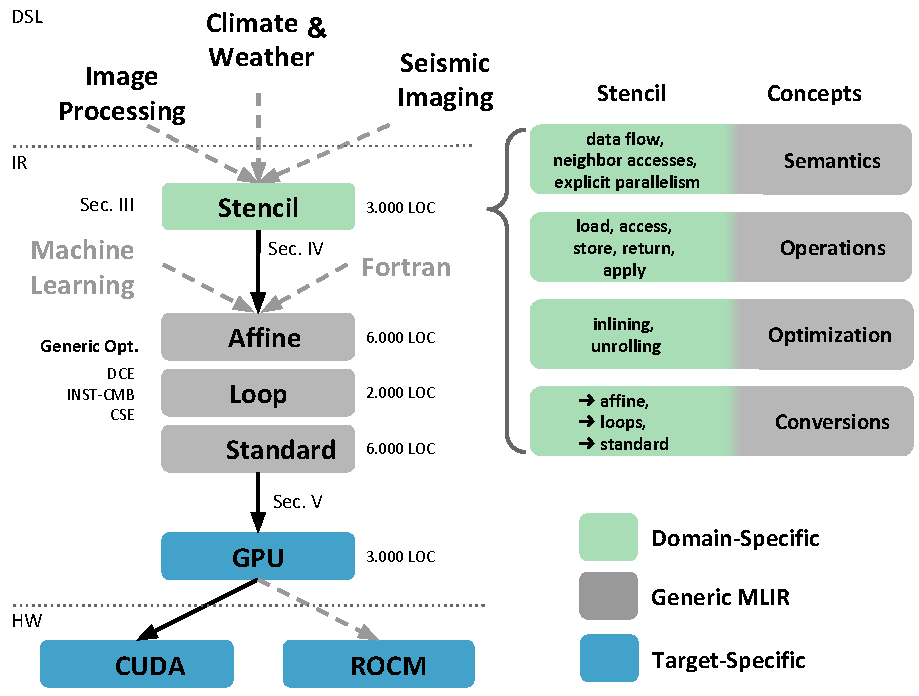
\includegraphics[width=\columnwidth]{overview.pdf}
% \caption{Our key idea visualized}
% \grosser{Replace this figure with your own drawing.}
% \end{figure}









%% Bibliography
\bibliographystyle{plain}
\bibliography{references}


\end{document}
